% Drawing 161-6/02-2 -- folder 161-6, batch 02, archive page 21 (PDF page 22).
% Transcription: dans la marge gauche, un icosaèdre dessiné en perspective : un contour hexagonal, quatre sommets intérieurs et les arêtes qui les joignent, quelques arêtes cachées en tirets.
% Kind: icosahedron in perspective (margin). Method 2 (schematic redraw from the facsimile). Status: partial.
% Notes: Small ink sketch of an icosahedron seen in perspective. Six vertices on the outline (a hexagon, its two upper right sides heavy) and four inside; every edge is drawn between these ten points: from the upper inner vertex to the three upper outline vertices, to the left outline vertex and to the central vertex; from the left outline vertex through the left inner vertex to the central vertex; from the left inner vertex up to the upper left vertex and down to the bottom vertex; from the central vertex to the right, lower right and bottom outline vertices; a fourth inner vertex at the right, joined by broken strokes to the upper right and lower right vertices and by a heavy stroke to the right vertex (hidden edges). 23 edges are drawn here; an icosahedron seen so shows more, and the page is too small and too heavily inked to tell every edge apart. Still differs: which strokes are edges is a reading; the bottom vertex is drawn double on the page (two close points) and single here. Redrawn 2026-11-10 (issue 128): to check again.
% Coordinates: 1 unit = 1 mm = 1/100 of the crop width (bbox in page fractions: [0.13, 0.25, 0.25, 0.32]).
% Redrawn by Claude (claude-fable-5-2), issue #128, 2026-11-10; not checked by a human; not compiled (no TeX in the session).
% Rights: reproduces part of the work -- behind RENDER_TRANSCRIPTS, never published by itself.
\documentclass[tikz,border=3pt]{standalone}
\usepackage{amsmath,amssymb}
\usetikzlibrary{patterns,arrows.meta}
\tikzset{pencil/.style={black!45}, struck/.style={black!35}, mpt/.style={circle,draw,inner sep=1.3pt}, pt/.style={circle,fill,inner sep=0.9pt}, opt/.style={circle,draw,fill=white,inner sep=1.1pt}}
\begin{document}
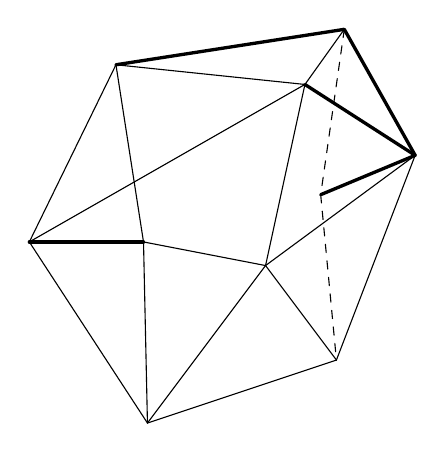
\begin{tikzpicture}[x=1mm,y=1mm,line cap=round,line join=round,font=\scriptsize]
\draw[very thick] (31,-17.5) -- (60,-13);
\draw[very thick] (60,-13) -- (69,-29);
\draw (69,-29) -- (59,-55);
\draw (59,-55) -- (35,-63);
\draw (35,-63) -- (20,-40);
\draw (20,-40) -- (31,-17.5);
\draw (31,-17.5) -- (55,-20);
\draw (55,-20) -- (60,-13);
\draw[very thick] (55,-20) -- (69,-29);
\draw (55,-20) -- (50,-43);
\draw (20,-40) -- (55,-20);
\draw[very thick] (20,-40) -- (34.5,-40);
\draw (34.5,-40) -- (50,-43);
\draw (31,-17.5) -- (34.5,-40);
\draw (34.5,-40) -- (35,-63);
\draw (50,-43) -- (69,-29);
\draw (50,-43) -- (59,-55);
\draw (50,-43) -- (35,-63);
\draw[dashed] (60,-13) -- (57,-34);
\draw[very thick] (57,-34) -- (69,-29);
\draw[dashed] (57,-34) -- (59,-55);
\end{tikzpicture}
\end{document}
